\documentclass[11pt]{book}

%%%%%%%%%%%%%%Include Packages%%%%%%%%%%%%%%%%%%%%%%%%%%
\usepackage{xcolor}
\usepackage{mathtools}
\usepackage[a4paper, total={6in, 8in}, margin=1in]{geometry}
\usepackage{amsmath}
\usepackage{amssymb}
\usepackage{paralist}
\usepackage{rsfso}
\usepackage{amsthm}
\usepackage{wasysym}
\usepackage[inline]{enumitem}   
\usepackage{hyperref}
\usepackage{tocloft}
\usepackage{wrapfig}
\usepackage{titlesec}
\usepackage{colortbl}
\usepackage{stackengine} 
\usepackage{csvsimple}
\usepackage{listings}
%%%%%%%%%%%%%%%%%%%%%%%%%%%%%%%%%%%%%%%%%%%%%%%%%%%%%%%%



%%%%%%%%%%%%%%%Code%%%%%%%%%%%%%%%%%%%%%%%%%%%%%%%%%%%%%
\definecolor{codegreen}{rgb}{0,0.6,0}
\definecolor{codegray}{rgb}{0.5,0.5,0.5}
\definecolor{codepurple}{rgb}{0.58,0,0.82}
\definecolor{backcolour}{rgb}{0.95,0.95,0.92}

\lstdefinestyle{mystyle}{
    backgroundcolor=\color{backcolour},   
    commentstyle=\color{codegreen},
    keywordstyle=\color{magenta},
    numberstyle=\tiny\color{codegray},
    stringstyle=\color{codepurple},
    basicstyle=\ttfamily\footnotesize,
    breakatwhitespace=false,         
    breaklines=true,                 
    captionpos=b,                    
    keepspaces=true,                 
    numbers=left,                    
    numbersep=5pt,                  
    showspaces=false,                
    showstringspaces=false,
    showtabs=false,                  
    tabsize=2
}
%%%%%%%%%%%%%%%%%%%%%%%%%%%%%%%%%%%%%%%%%%%%%%%%%%%%%%%%




%%%%%%%%%%%%%%%Chapter Setting%%%%%%%%%%%%%%%%%%%%%%%%%%
\definecolor{gray75}{gray}{0.75}
\newcommand{\hsp}{\hspace{20pt}}
\titleformat{\chapter}[hang]{\Huge\bfseries}{\thechapter\hsp\textcolor{gray75}{$\mid$}\hsp}{0pt}{\Huge\bfseries}
%%%%%%%%%%%%%%%%%%%%%%%%%%%%%%%%%%%%%%%%%%%%%%%%%%%%%%%%

%%%%%%%%%%%%%%%%%Theorem environments%%%%%%%%%%%%%%%%%%%
\newtheoremstyle{break}
  {\topsep}{\topsep}%
  {\itshape}{}%
  {\bfseries}{}%
  {\newline}{}%
\theoremstyle{break}
\theoremstyle{break}
\newtheorem{axiom}{Axiom}
\newtheorem{thm}{Theorem}[section]
\renewcommand{\thethm}{\arabic{section}.\arabic{thm}}
\newtheorem{lem}{Lemma}[thm]
\newtheorem{prop}[lem]{Proposition}
\newtheorem{corL}{Corollary}[lem]
\newtheorem{corT}[lem]{Corollary}
\newtheorem{defn}{Definition}[corL]
\newenvironment{indEnv}[1][Proof]
  {\proof[#1]\leftskip=1cm\rightskip=1cm}
  {\endproof}
%%%%%%%%%%%%%%%%%%%%%%%%%%%%%%%%%%%%%%%%%%%%%%%%%%%%%%


%%%%%%%%%%%%%%%%%%%%%%%Integral%%%%%%%%%%%%%%%%%%%%%%%
\def\upint{\mathchoice%
    {\mkern13mu\overline{\vphantom{\intop}\mkern7mu}\mkern-20mu}%
    {\mkern7mu\overline{\vphantom{\intop}\mkern7mu}\mkern-14mu}%
    {\mkern7mu\overline{\vphantom{\intop}\mkern7mu}\mkern-14mu}%
    {\mkern7mu\overline{\vphantom{\intop}\mkern7mu}\mkern-14mu}%
  \int}
\def\lowint{\mkern3mu\underline{\vphantom{\intop}\mkern7mu}\mkern-10mu\int}
%%%%%%%%%%%%%%%%%%%%%%%%%%%%%%%%%%%%%%%%%%%%%%%%%%%%%%



\newcommand{\R}{\mathbb{R}}
\newcommand{\N}{\mathbb{N}}
\newcommand{\Z}{\mathbb{Z}}
\newcommand{\Q}{\mathbb{Q}}
\newcommand{\C}{\mathbb{C}}
\newcommand{\T}{\mathcal{T}}
\newcommand{\M}{\mathcal{M}}
\newcommand{\Symm}{\text{Symm}}
\newcommand{\Alt}{\text{Alt}}
\newcommand{\Int}{\text{Int}}
\newcommand{\Bd}{\text{Bd}}
\newcommand{\Power}{\mathcal{P}}
\newcommand{\ee}[1]{\cdot 10^{#1}}
\newcommand{\spa}{\text{span}}
\newcommand{\sgn}{\text{sgn}}
\newcommand{\degr}{\text{deg}}
\newcommand{\pd}{\partial}
\newcommand{\that}[1]{\widetilde{#1}}
\newcommand{\lr}[1]{\left(#1\right)}
\newcommand{\vmat}[1]{\begin{vmatrix} #1 \end{vmatrix}}
\newcommand{\bmat}[1]{\begin{bmatrix} #1 \end{bmatrix}}
\newcommand{\pmat}[1]{\begin{pmatrix} #1 \end{pmatrix}}
\newcommand{\rref}{\xrightarrow{\text{row\ reduce}}}
\newcommand{\txtarrow}[1]{\xrightarrow{\text{#1}}}
\newcommand\oast{\stackMath\mathbin{\stackinset{c}{0ex}{c}{0ex}{\ast}{\Circle}}}


\newcommand{\note}{\color{red}Note: \color{black}}
\newcommand{\remark}{\color{blue}Remark: \color{black}}
\newcommand{\example}{\color{green}Example: \color{black}}
\newcommand{\exercise}{\color{green}Exercise: \color{black}}

%%%%%%%%%%%%%%%%%%%%%%Roman Number%%%%%%%%%%%%%%%%%%%%%%%
\makeatletter
\newcommand*{\rom}[1]{\expandafter\@slowromancap\romannumeral #1@}
\makeatother
%%%%%%%%%%%%%%%%%%%%%%%%%%%%%%%%%%%%%%%%%%%%%%%%%%%%%%%%%

%%%%%%%%%%%%table of contents%%%%%%%%%%%%%%%%%%%%%%%%%%%%
\setlength{\cftchapindent}{0em}
\cftsetindents{section}{2em}{3em}

\renewcommand\cfttoctitlefont{\hfill\huge\bfseries}
\renewcommand\cftaftertoctitle{\hfill\mbox{}}

\setcounter{tocdepth}{2}
%%%%%%%%%%%%%%%%%%%%%%%%%%%%%%%%%%%%%%%%%%%%%%%%%%%%%%%%%


%%%%%%%%%%%%%%%%%%%%%Footnotes%%%%%%%%%%%%%%%%%%%%%%%%%%%
\newcommand\blfootnote[1]{%
  \begingroup
  \renewcommand\thefootnote{}\footnote{#1}%
  \addtocounter{footnote}{-1}%
  \endgroup
}
%%%%%%%%%%%%%%%%%%%%%%%%%%%%%%%%%%%%%%%%%%%%%%%%%%%%%%%%%

%%%%%%%%%%%%%%%%%%%%%Section%%%%%%%%%%%%%%%%%%%%%%%%%%%%%
\makeatletter
\def\@seccntformat#1{%
  \expandafter\ifx\csname c@#1\endcsname\c@section\else
  \csname the#1\endcsname\quad
  \fi}
\makeatother
%%%%%%%%%%%%%%%%%%%%%%%%%%%%%%%%%%%%%%%%%%%%%%%%%%%%%%%%%

%%%%%%%%%%%%%%%%%%%%%%%%%%%%%%%%%%%Enumerate%%%%%%%%%%%%%%
\makeatletter
% This command ignores the optional argument 
% for itemize and enumerate lists
\newcommand{\inlineitem}[1][]{%
\ifnum\enit@type=\tw@
    {\descriptionlabel{#1}}
  \hspace{\labelsep}%
\else
  \ifnum\enit@type=\z@
       \refstepcounter{\@listctr}\fi
    \quad\@itemlabel\hspace{\labelsep}%
\fi}
\makeatother
\parindent=0pt
%%%%%%%%%%%%%%%%%%%%%%%%%%%%%%%%%%%%%%%%%%%%%%%%%%%%%%%%%%


\begin{document}

	\begin{titlepage}
		\begin{center}
			\vspace*{1cm}
			\Huge \color{red}
				\textbf{Lab 6 Report}\\
			\vspace{0.5cm}			
			\Large \color{black}
				Math 391 - Introduction to Modern Physics Lab\\
				Professor Wayne Lau\\	
				University of Michigan\\
			\vspace{3cm}

			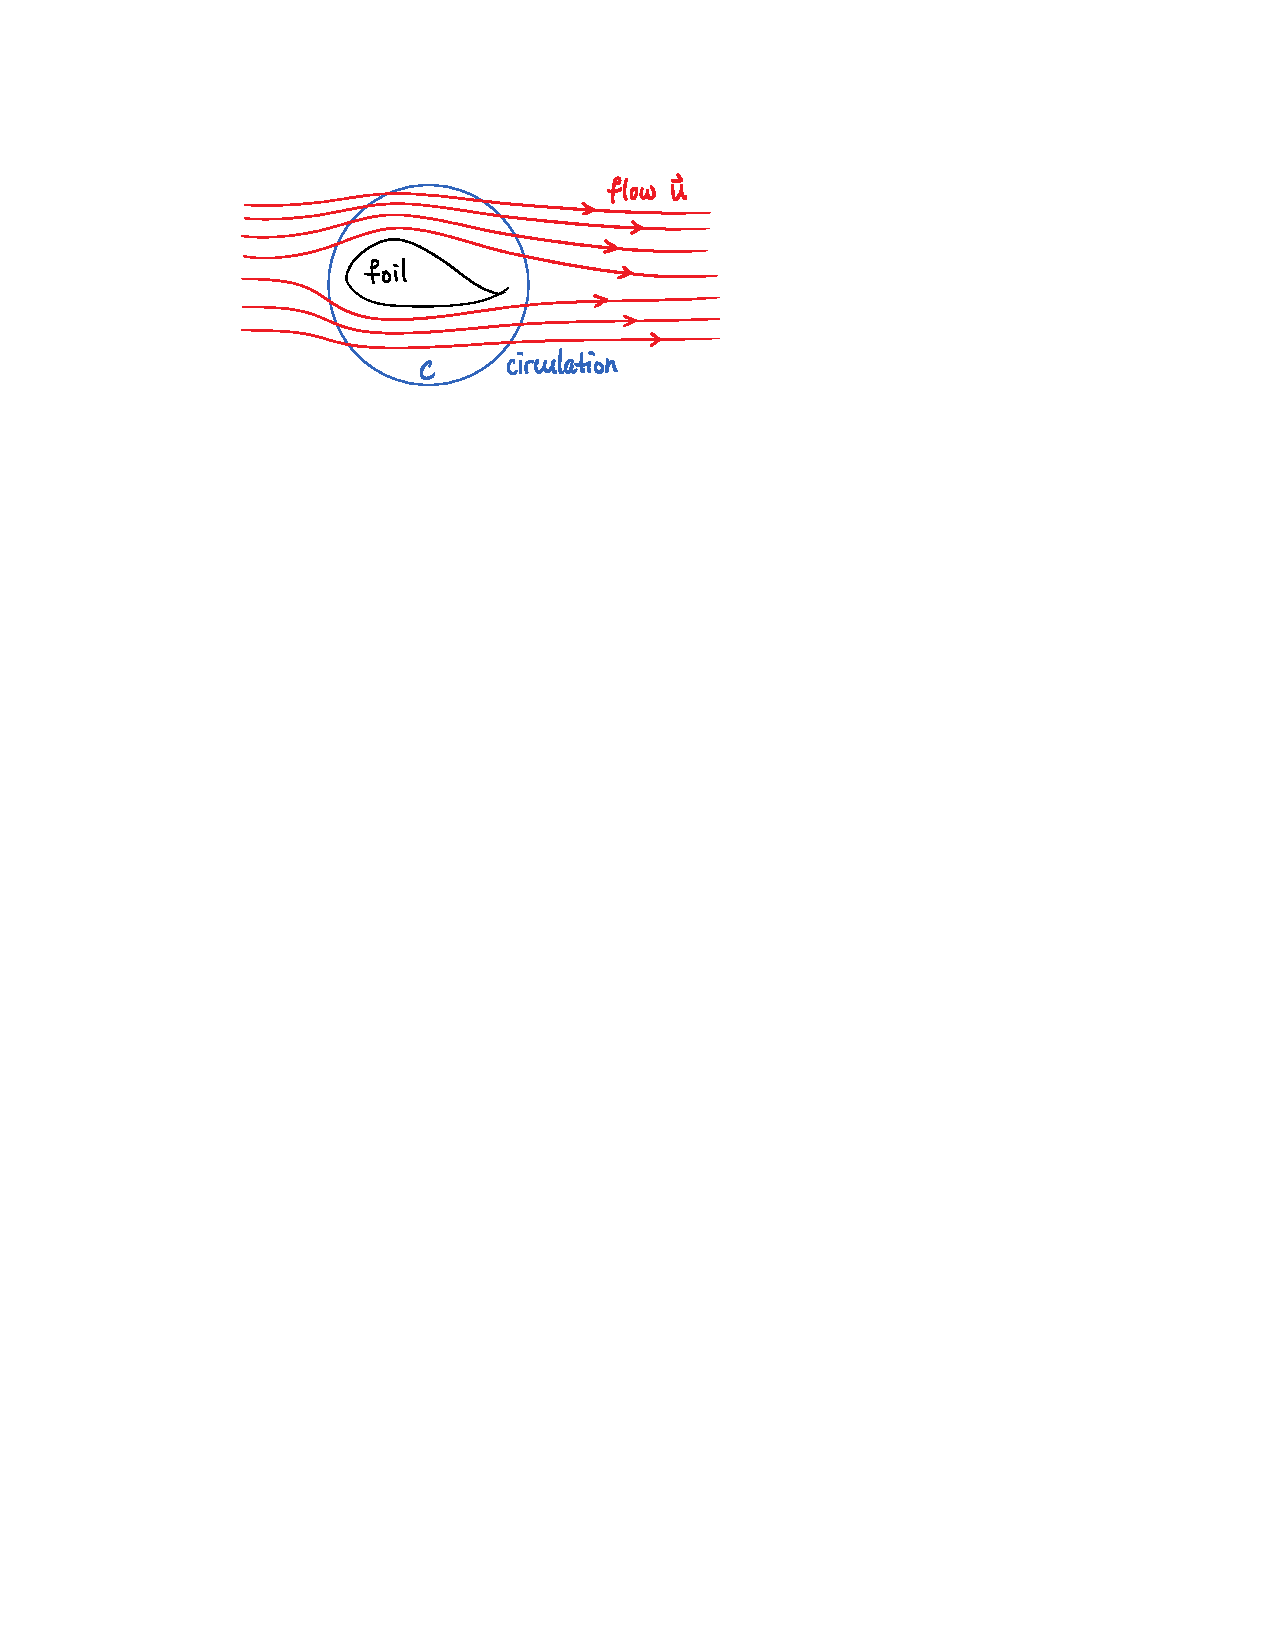
\includegraphics[scale=1.29]{circulation.pdf}\\
			\color{gray}The Kutta–Joukowski Lift Theorem\color{black}
			
			
			\vspace{5cm}
			\LARGE
				\textbf{Jinyan Miao}\\
				\hfill\break
				\LARGE Fall 2022\\
			\vspace{1cm}

		\vspace*{\fill}
		\end{center}			
	\end{titlepage}


\newpage
\tableofcontents
\addtocontents{toc}{~\hfill\textbf{Page}\par}


\setcounter{chapter}{6}
\chapter*{Lab 6 - Spectroscopy \\of Atomic Hydrogen and Deuterium }
\section{Introduction}
The observations in optical spectroscopy in the 19th century led to the development of quantum theory. Among those observations, the line spectrum for hydrogen atoms was one of the most important ones. In the visible region, the line spectrum, showed by Johann Balmer, is well described by the geometric series:
\begin{align}
\lambda = G \frac{n^2}{n^2 - 4} \qquad \forall	 n \in \N - \{1,2\}
\end{align}
where $G$ is an empirical constant. In 1889, Johannes Rydberg proposed a more general expression for the spectral line of hydrogen atom:
\begin{align}
\frac{1}{\lambda} = R_H \left( \frac{1}{n_1^2} - \frac{1}{n_2^2}\right) \qquad n_2 > n_1 
\end{align}
and the Balmer series characterized by (6.1) is a special case characterized by (6.2) when $n_1 = 2$. The Rydberg constant is given by the following:
\begin{align}
R_H = \left( \frac{1}{4\pi \epsilon_0}\right)^2 \frac{me^4}{4\pi \hbar^3 c} = 10.9737316 \,\text{micron}^{-1}
\end{align}
Here the spectral lines predicted by (6.2) are given by the followings:
\begin{center}
\begin{tabular}{|c|c|c|}
\hline
Line Designation & Transition & Wavelength (nm) \\
\hline 
$H_\alpha$ & $3\to 2$ & 656.27 \\
\hline
$H_\beta$ & $4\to 2$ & 486.13 \\
\hline
$H_\gamma$ & $5\to 2$ & 434.05 \\
\hline
$H_\delta$ & $6\to 2$ & 410.17 \\
\hline
$H_\epsilon$ & $7\to 2$ & 397.01 \\
\hline
$H_\zeta$ & $8\to 2$ & 388.91 \\
\hline
\end{tabular}
\end{center}
Note that $R_H$ is the value that would be appropriate if the nucleus is fixed. In practice, the mass of the electron should be replaced by the reduced mass $m_eM_N /(m_e+M_N)$ where $M_N$ is the mass of the nucleus. Thus the spectrum has a dependence on the nucleus mass. Hence one can find the ratio between the electron mass and the proton mass by evaluating the frequency shift $\Delta \nu = \nu_H - \nu_D$ of the alpha lines in the hydrogen atom spectrum and the deuterium atom spectrum:
\begin{align}
\frac{\Delta \nu}{\nu_H} = \left( 1 - \frac{m_e}{M_D}\right) - \left( 1 - \frac{m_e}{M_P}\right) \approx \frac{m_e}{2M_P}
\end{align}
where $M_D$ is the nucleus mass of the deuterium atom, and we approximate $M_D$ by $2M_P$, with $M_P$ being the mass of a proton. \\

In Lab 6 of Physics 391, we measure six lines of the Balmer series ranging from $656\, nm$ to $388\, nm$ with a hydrogen discharge tube as the light source. We then compare our results to the predicted values given by (6.2) and used our data to estimate $R_H$. The estimated $R_H$ is given by $11.0624 \pm 0.0742 \, \text{micron}^{-1}$, capturing the theoretical value given by (6.3). We then use the same setup to make precise measurements on the alpha lines for both the hydrogen and the deuterium atom, estimate the frequency shift, and hence the electron-proton mass ratio via (6.4).\\


\hfill\break
\section{Experimental setup} 
First, we measure the wavelengths of the first six lines of the Balmer series using a hydrogen discharge tube as a light source and a spectrometer manufactured by Vernier. The light sources are narrow glass gas discharge tubes that are mounted in a vertical support which supplies the voltage. We adjust the spectrometer exposure for each line to optimize the accuracy, and the readout is performed by Logger Pro which controls all aspects of the data acquisition and logging. We obtain one set of data that contains wavelengths and the corresponding detected intensities of the light from the hydrogen discharge tube. Then we use a similar setup and use a deuterium discharge tube to obtain data for estimating the frequency shift. We take a total of 20 different data runs, 5 for hydrogen, 5 for deuterium, then again 5 for hydrogen and 5 for deuterium.\\


\newpage
\section{Visualizing the data}
For the measurement of the wavelengths of the Balmer series, we make 6 measurements, with different exposure of the spectrometer, and obtain the followings:
\begin{center}
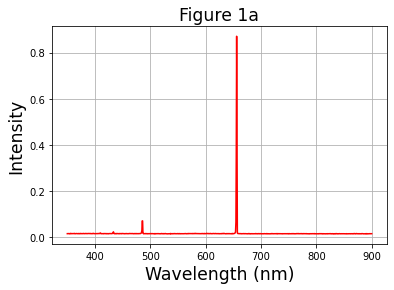
\includegraphics[scale=0.55]{1a}
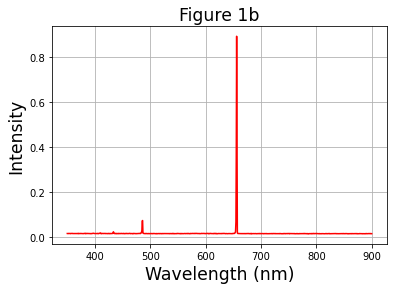
\includegraphics[scale=0.55]{1b}
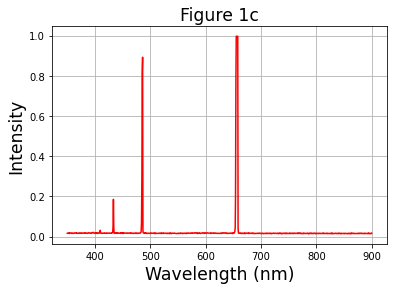
\includegraphics[scale=0.55]{1c}
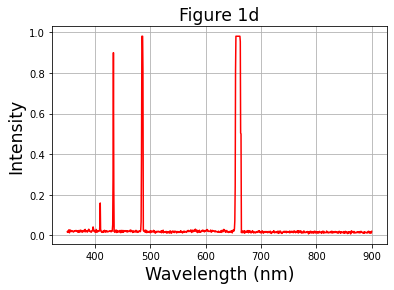
\includegraphics[scale=0.55]{1d}
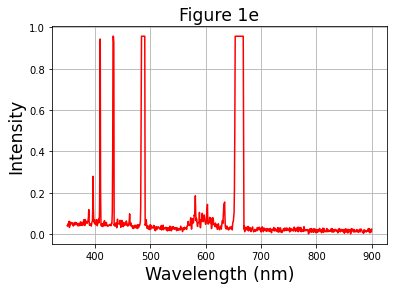
\includegraphics[scale=0.55]{1e}
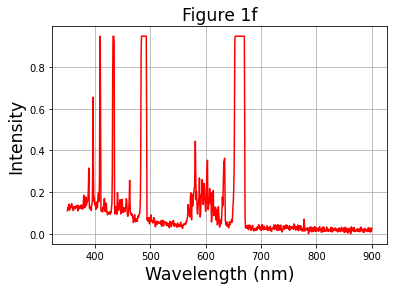
\includegraphics[scale=0.55]{1f}
\end{center}
\newpage
We truncate each dataset and limit the wavelengths to be around the wavelengths of the Balmer series, and concatenate into a single data set, obtaining the following figure:
\begin{center}
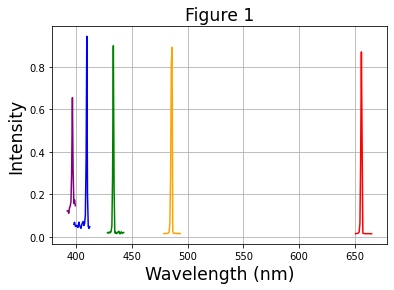
\includegraphics[scale=0.55]{fig1}
\end{center} 
Each line in Fig. 1 represents a spectral line in the Balmer series.\\

We then estimate the wavelengths of the peaks of the intensity in the truncated-concatenated dataset via mean position:
\begin{align*}
\bar{x} = \frac{\sum_i x_i y_i}{\sum_i y_i}
\end{align*} 
where $\{x_i\}$ is the set of wavelengths near the local peak and $\{y_i\}$ is the associated set of intensities. As a result, we obtain the estimated wavelengths of the Balmer series:
\begin{center}
\begin{tabular}{|c|c|c|c|}
\hline
Line Designation & Estimated $\lambda$ (nm) & Theoretical $\lambda$ (nm)& Deviation \\
\hline 
$H_\alpha$ & 656.22 & 656.27 & 0.01$\%$ \\
\hline
$H_\beta$ & 485.66 & 486.13 & 0.10$\%$\\
\hline
$H_\gamma$ & 433.86 & 434.05 & 0.04$\%$\\
\hline
$H_\delta$ & 407.33 & 410.17 & 0.69$\%$\\
\hline
$H_\epsilon$ & 395.97 & 397.01 & 0.26$\%$\\
\hline
$H_\zeta$ & 388.21 & 388.91 & 0.17$\%$\\
\hline
\end{tabular}
\end{center}
Note that the deviation from the theoretical values is higher for those with lower wavelengths, this is because the lower wavelengths have smaller intensities, and hence it is more difficult for the equipment to make precise measurements.\\

We plot $1/\lambda$ over $1/4 - 1/n^2$ where $n$ is the $n_2$ of the spectral line given in (6.2):
\begin{center}
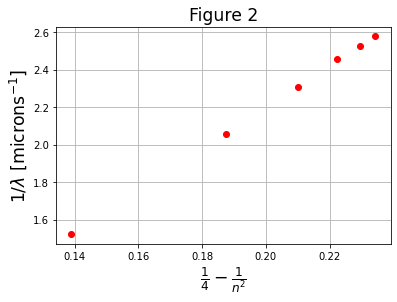
\includegraphics[scale=0.55]{2}
\end{center}


For the comparison between the hydrogen atom alpha line and deuterium alpha line, we group the first 5 hydrogen data runs and the first 5 deuterium data runs as experiment 1, and the rest as experiment 2. Then we calculate the average intensity recorded for each wavelength. 
\begin{center}
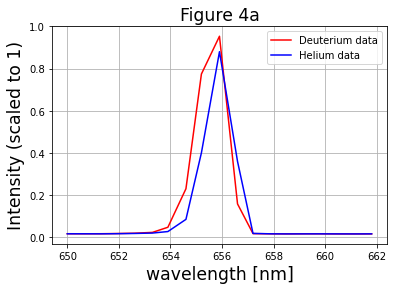
\includegraphics[scale=0.55]{4a}
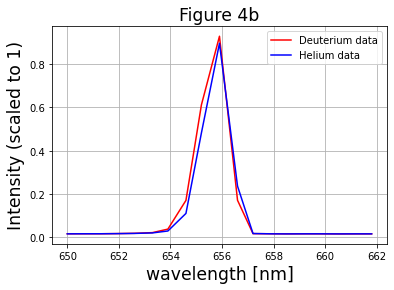
\includegraphics[scale=0.55]{4b}
\end{center}
Here Fig. 4a displays data for experiment 1, and Fig. 4b displays data for experiment 2. Note that in both experiments, the peaks of the deuterium spectra have smaller wavelengths.\\


\hfill\break
\hfill\break

\section{Analyzing the data}
\subsection{Estimation of the Rydberg constant}
Here we perform a linear fit $y = mx+b$ to the dataset displayed in Fig. 2:
\begin{center}
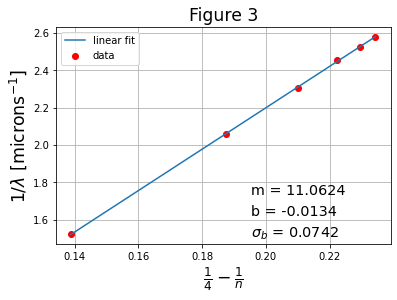
\includegraphics[scale=0.55]{3}
\end{center}
According to (6.2), $R_H$ is given by the slope of the linear fit, in our case, we see that $R_H$ is estimated to be $11.0624 \, \text{micron}^{-1}$, with a standard deviation $0.0742$. Note that the y-axis interception $b = -0.0134$ is negligible, hence confirming the validity of (6.2). Moreover, the theoretical value of $R_H$ is around $10.9737$, and we have:
\begin{align*}
\frac{|11.0624 - 10.9737|}{0.0742} = 1.195
\end{align*}
hence the theoretical value of $R_H$ is captured within 3$\sigma$ from our estimation, suggesting that the theoretical value is well-predicted by our data, and our data gives a good approximation to the true $R_H$.

\subsection{Comparison of deuterium and hydrogen alpha lines}
First, we perform individual Gaussian fit to the data via the following model:
\begin{align}
y_H = a_H  + b_H e^{-\frac{(x-(656-\delta_H))^2}{2\sigma_H^2}}\qquad\qquad y_D = a_D  + b_D e^{-\frac{(x-(656-\delta_D))^2}{2\sigma_D^2}}
\end{align}
where $y_H,y_D$ are the intensities of the hydrogen spectrum and the deuterium spectrum, respectively, $a_H,a_D,b_H, b_D$ are linear parameters, $\delta_H$, $\delta_D$, $\sigma_H$, $\sigma_D$ are non-linear parameters, and $x$ is the wavelengths. For individual fit, we obtain the followings:
\begin{center}
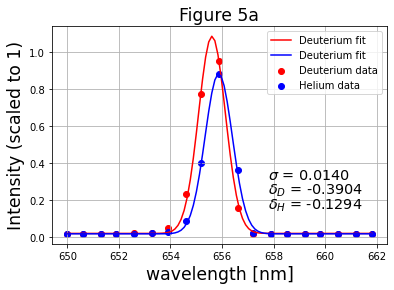
\includegraphics[scale=0.55]{5a}
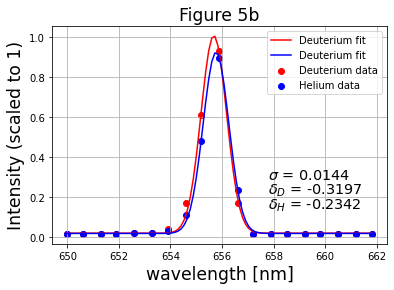
\includegraphics[scale=0.55]{5b}
\end{center}
Fig. 5a displays the data and the fit for experiment 1, and Fig. 5b displays the data and the fit for experiment 2. For both experiments, we see that the peaks for the deuterium spectrum have lower wavelengths. More specifically, we can compute:
\begin{align*}
\delta_H - \delta_D &= 0.2610\, nm
\tag{experiment 1}\\
\delta_H - \delta_D &= 0.0855\, nm \tag{experiment 2}
\end{align*} 
and the standard deviation for $\delta_H - \delta_D$
\begin{align*}
\sigma &= \sqrt{\sigma_{D}^2 + \sigma_{H}^2} = 0.0140\,nm  \tag{experiment 1}\\
\sigma &= \sqrt{\sigma_{D}^2 + \sigma_{H}^2} = 0.0144\, nm  \tag{experiment 2}
\end{align*}
The theoretical difference $\Delta =\delta_H - \delta_D$ is $0.18\, nm$, and we see that such theoretical value is not captured within $3\sigma$ by either of the two experiments. In particular, experiment 1 gives an overestimation ($5.78\sigma$ away) of the true $\Delta$, while experiment 2 gives a underestimation ($6.6\sigma$ away) of $\Delta$. Moreover, we note that the estimated value of $\delta_D$ and $\delta_H$ in both experiments are less than zero, but the true value of $\delta_D$ and $\delta_H$ should be greater than zero as predicted by (6.2), this is a systematic error. One possible cause of such an error is the change in temperature of the hydrogen discharger tube, and the calibration of the equipment in the experiments. \\

We then perform a joint fitting of the Gaussian curves in the two experiments. For each experiment, we again fit the data via (6.5), but with $\sigma_D = \sigma_H$, and we obtain the following results:
\begin{center}
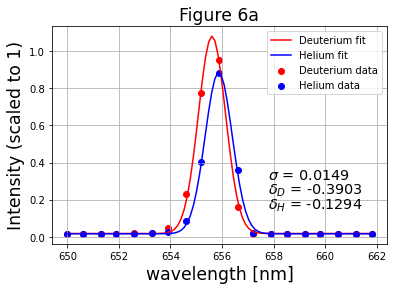
\includegraphics[scale=0.55]{6a}
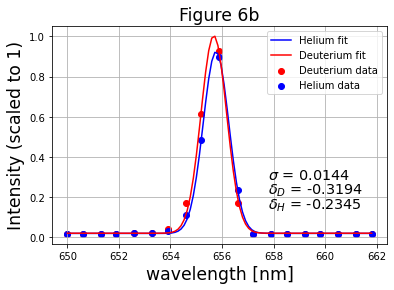
\includegraphics[scale=0.55]{6b}
\end{center}
Notice that the difference between this fit and the previous one is minimal. Experiment 1 gives an underestimation of the true $\Delta$, and experiment 2 gives an overestimation of the true $\Delta$. 
\begin{center}
\begin{tabular}{|c|c|c|c|}
\hline
& estimated $\Delta = \delta_H - \delta_D$ & $\sigma$ & difference from true $\Delta$\\
\hline
Experiment 1 & 0.2608 & 0.0149 & $5.7\sigma$\\ 
\hline
Experiment 2 & 0.0849 & 0.0144 & $6.6\sigma$\\
\hline
\end{tabular}
\end{center}

\subsection{Estimation of electron-proton mass ratio}
Rearranging (6.4), we obtain:
\begin{align*}
\frac{m_e}{M_P} = 2 \cdot \frac{\Delta \nu}{\nu_H}
\end{align*}
and we obtain the following results:
\begin{center}
\begin{tabular}{|c|c|c|}
\hline
& $m_e/M_P$ (via joint fitting) & st. dev. (via joint fitting)\\
\hline
Experiment 1 & 0.000795 & 0.056959 \\
\hline
Experiment 2 & 0.000259 & 0.169572 \\
\hline
\end{tabular}\\
\hfill\break
\hfill\break
\begin{tabular}{|c|c|c|}
\hline
& $m_e/M_P$ (via individual fitting) & st. dev. (via individual fitting)\\
\hline
Experiment 1 & 0.000796 & 0.053458 \\
\hline
Experiment 2 & 0.000261 & 0.168148\\
\hline
\end{tabular}
\end{center}
The true ratio between electron and proton mass is given by $0.000544$. The standard deviation in our estimation is large, as a result, the true value is captured within $1\sigma$ from our estimated values in alll cases. This shows that the ratio between electron mass and proton mass is statistically well predicted from our experimental results. 


\section{Summary}
In Lab 6 of Physics 391, we measure the wavelengths of the Balmer series for hydrogen atoms, and we have verified the validity of equation (6.2). We also estimated the Rydberg constant to be around $11.0624 \pm 0.0742\, \text{micron}^{-1}$, successfully capturing the true value of $R_H$. Moreover, we measured the frequency shift of the alpha line between the deuterium atom and hydrogen atom due to the effect of reduced mass. There is a systematic error present in our data, possibly due to the temperature change in the hydrogen discharging tube and some other equipment calibration issues. Lastly, we estimated the ratio of the electron mass over the proton mass, and the estimation captures the true ratio of the two masses. 



\newpage
\section{Code}
The code for computing statistics of the data sets is attached.
\lstset{style=mystyle}
\lstinputlisting[language=Python]{code.py}


\end{document}